\section{Running SS}
SS can be run from a DOS window in a directory containing the file SS3.EXE (or a path to SS3.EXE) and the necessary input files.  Simply type SS3 at the DOS prompt.  This will start the executable and the first step will be to open and read the file named starter.ss which contains necessary run information.

As with all ADMB-based programs, switches are typed immediately after a space.  For example, SS3 –nohess, would run SS3 without calculating the Hessian matrix.

\subsection{Example of DOS batch input file}
One file management approach is to put SS3.EXE in its own folder (example:  C:\textbackslash SS\_model) and to put your input files in separate folder (example:  C:\textbackslash My Documents \textbackslash SS\_runs).  Then a DOS batch file in the SS\_runs folder can be run at the command line to start SS3.EXE.  All output will appear in SS\_runs folder.

A DOS batch file (e.g. SS.bat) might contain some explicit ADMB commands, some implicit commands, and some DOS commands:

\begin{center}
	\begin{longtable}{ p{13cm} }
		c: \textbackslash SS\_model \textbackslash ss3.exe -cbs 5000000000 -gbs 50000000000 \%1 \%2 \%3 \%4 \\
		del ss3.r0*\\
		del ss3.p0*\\
		del ss3.b0*\\
	\end{longtable}
\end{center}

In this batch file, the –cbs and –gbs arguments allocate a large amount of memory for SS to use (you may need to edit these for your computer and SS configuration), and the \%1, \%2 etc. allows passing of command line arguments such as –nox or –nohess.  You add more items to the list of \% arguments as needed.

An easy way to start a command line in your current directory (SS\_runs) is to create a shortcut to the DOS command line prompt.  The shortcut’s target would be:

\begin{center}
	\begin{longtable}{p{13cm}}
		\%SystemRoot\%\textbackslash system32 \textbackslash cmd.exe\\
		And it would start in \%CURRDIR\%\\
	\end{longtable}
\end{center}

\subsubsection{Simple Batch}
This first example relies upon having a set of prototype files that can be renamed to starter.ss and then used to direct the running of SS.  The example also copies one of the output files to save it from being overwritten.  This sequence is repeated 3 times here and can be repeated an unlimited number of times.  The batch file can have any name with the .bat extension, and there is no particular limit to the DOS commands invoked.  Note that brief output from each run will be appended to cumreport.sso (see below).

\begin{center}
	\begin{longtable}{p{13cm}}
		del ss3.cor\\
		del ss3.std\\
		copy starter.r01 starter.ss\\
		c:\textbackslash admodel\textbackslash ss\textbackslash ss3.exe -sdonly\\
		copy ss3.std ss-std01.txt\\
		copy starter.r01 starter.ss\\
		c:\textbackslash admodel\textbackslash ss\textbackslash ss3.exe -sdonly\\
		copy ss3.std ss-std02.txt\\
	\end{longtable}
\end{center}

\subsubsection{Complicated Batch}
This second example processes 25 dat files from a different directory, each time using the same ctl and nam file.  The loop index is used in the file names, and the output is searched for particular keywords to accumulate a few key results into the file SUMMARY.TXT.  Comparable batch processing can be accomplished by using R or other script processing programs.

\begin{center}
	\begin{longtable}{p{13cm}}
		del summary.txt\\
		del ss3-report.txt\\
		copy /Y runnumber.zero runnumber.ss3\\
		FOR /L \%\%i IN (1,1,25) DO (\\
		copy /Y ..\textbackslash MakeData\textbackslash A1-D1-\%\%i.dat  Asel.dat\\
		del ss3.std\\
		del ss3.cor\\
		del ss3.par\\
		c:\textbackslash admodel\textbackslash ss\textbackslash ss3.exe\\
		copy /Y ss3.par A1-D1-A1-\%\%i.par\\
		copy /Y ss3.std A1-D1-A1-\%\%i.std\\
		find "Number" A1-D1-A1-\%\%i.par >> Summary.txt\\
		find "hessian" ss3.cor >> Summary.txt)\\	
	\end{longtable}
\end{center}

\subsubsection{Batch Using PROFILEVALUES.SS}
This example will run a profile on natural mortality and spawner-recruitment steepness, of course.  Edit the control file so that the natural mortality parameter and steepness parameter lines have the phase set to –9999.  Edit STARTER.SS to refer to this control file and the appropriate data file.

\begin{center}
	\begin{longtable}{p{13cm}}		
		Create a PROFILEVALUES.SS file\\
		2	\# number of parameters using profile feature\\
		0.16	\# value for first selected parameter when runnumber equals 1\\
		0.35	\# value for second selected parameter when runnumber equals 1\\
		0.16	\# value for first selected parameter when runnumber equals 2\\
		0.40	\# value for second selected parameter when runnumber equals 2\\
		0.18	\# value for first selected parameter when runnumber equals 3\\
		0.40	\# value for second selected parameter when runnumber equals 3\\
		etc.;  make it as long as you like.\\
	\end{longtable}
\end{center}

Create a batch file that looks something like this.  Or make it more complicated as in the example above.

\begin{center}
	\begin{longtable}{p{15cm}}		
		del cumreport.sso\\
		copy /Y runnumber.zero runnumber.ss  \% so you will start with runnumber=0 \\
		C:\textbackslash SS3\textbackslash ss3.exe \\
		C:\textbackslash SS3\textbackslash ss3.exe \\
		C:\textbackslash SS3\textbackslash ss3.exe \\
	\end{longtable}
\end{center}

Repeat as many times as you have set up conditions in the PROFILEVALUES.SS file.
The summary results will all be collected in the cumreport.sso file.  Each step of the profile will have an unique Runnumber and its output will include the values of the natmort and steepness parameters for that run.

\subsubsection{Re-Starting a Run}
SS model runs can be restarted from a previously estimated set of parameter values.  In the starter.ss file, enter a value of 1 on the first numeric input line.  This will cause SS to read the file ss3.par and use these parameter values in place of the initial values in the control file.  This option only works if the number of parameters to be estimated in the new run is the same as the number of parameters in the previous run because only actively estimated parameters are saved to the file ss3.par.  The file ss3.par can be edited with a text editor, so values can be changed and rows can be added or deleted.  However, if the resulting number of elements does not match the setup in the control file, then unpredictable results will occur.  Because ss3.par is a text file, the values stored in it will not give exactly the same initial results as the run just completed.  To achieve greater numerical accuracy, SS can also restart from ss3.bar which is the binary version of ss3.par.  In order to do this, the user must make the change described above to the starter.ss file and must also enter –binp ss3.bar as one of the command line options.

\subsubsection{Debugging Tips}
When SS input files are causing the program to crash or fail to produce sensible results, there are a few steps that can be taken to diagnose the problem.  Before trying the steps below, examine the ECHOINPUT.SSO file.  It is highly annotated, so you should be able to see if SS is interpreting your input files as you intended.

\begin{enumerate}
	\item Set the turn\_off\_phase switch to 0 in the STARTER.SS file.  This will cause the mode to not attempt to adjust any parameters and simply converges a dummy parameter.  It will still produce a REPORT.SSO file, which can be examined to see what has been calculated from the initial parameter values.
	\item Turn the verbosity level to 2 in the STARTER.SS file.  This will cause the program to display the value of each likelihood component to the screen on each iteration.  So it the program is creating an illegal computation (e.g. divide by zero), it may show you which likelihood component contains the problematic calculation.  If the program is producing a REPORT.SSO file, you may then see which observation is causing the illegal calculation.
	\item Run the program with the command SS3 >>SSpipe.txt.  This will cause all screen display to go to the specified text file (note, delete this file before running because it will be appended to).  Examination of this file will show detailed statements produced during the reading and preprocessing of input files.
	\item CHECKUP.SSO:  This file can be written during the first iteration of the program.  It contains details of selectivity and other calculations as an aid to debugging model problems. 
	\item If SS fails to achieve a proper Hessian it exits without writing the detailed outputs in the FINAL\_SECTION.  If this happens, you can do a run with the –nohess option so you can view the report.sso to attempt to diagnose the problem.
\end{enumerate}

\subsubsection{Keyboard Tips}
Typing “N” during a run will cause ADMB to immediately advance to the next phase of estimation.

Typing “Q”  during a run will cause ADMB to immediately go to the final phase.  This bypasses estimation of the Hessian and will produce all of the SS outputs, which are coded in the FINAL\_SECTION.

\subsubsection{Running MCMC}
 Run SS3
 \begin{itemize}
 	\item This gives MPD estimates, report file, Hessian matrix and the .cor file
 	\item (Recommended) Look for parameters stuck on bounds which will degrade efficiency of MCMC implementation
 	\item (Recommended) Look for very high correlations that may degrade the efficiency of MCMC implementation
 \end{itemize}
 
\noindent Run SS3 with arguments -mcmc xxxx -mcsave yyyy
 \begin{itemize}
 	\item Where: xxxx is the number of iterations for the chain, and yyyy is the thinning interval (1000 is a good place to start)
 	\item MCMC chain starts at the MPD values
 	\item (Recommended) Remove existing .psv files in run directory to generate a new chain.
 	\item (Recommended) Set DOS run detail switch in starter file to 0; reporting to screen will dramatically slow MCMC progress
 	\item (Optional) Add -nohess to use the existing Hessian file without re-estimating
 	\item (Optional) To start the MCMC chain from specific values change the par file; run the model with estimation, adjust the par file to the values that the chain should start from, change within the starter file for the model to begin from the par file, and call the MCMC function using ss3 –mcmc xxxx – mcsave yyyy -nohess –noest.
 	\item (Optional) Add -noest -nohess and modify starter file so that run will now start from the converged (or modified) parameter estimates in "ss3.par"
 \end{itemize}
	
\noindent Run SS3 with argument -mceval
\begin{itemize}
	\item This generates the posterior output files.
	\item (Optional) Modify starter file entries to add a burn-in and thinning interval above and beyond the ADMB thinning interval applied at run time.
	\item (Recommended) MCMC always begins with the MPD values and so a burn-in >0 should always be used.
	\item This step can be repeated for alternate forecast options (e.g. catch levels) without repeating step 2.
\end{itemize}

\noindent (Optional) Run SS3 with arguments -mcr -mcmc xxxx -mcsave yyyy ...
\begin{itemize}
	\item This restarts and extends an uninterrupted chain previously completed (note that any intermediate runs without the -mcr command in the same directory will break this option).
\end{itemize}

\noindent NOTES:\\
When SS switches to MCMC or MCEVAL mode, it sets all the bias adjustment factors to 1.0 for any years with recruitment deviations defined.  SS does not create a report file after completing MCMC because it would show values based on the last MCMC step.

\subsubsection{Using R To View Model Output}
A collection of functions developed as a package, r4ss, for the statistical software R has been created to explore SS model output.  The functions include tools for summarizing and plotting results, manipulating files, visualizing model parameterizations, and various other tasks.  Currently, information on the code can be found at code.goole.com/p/r4ss which facilities exploration of the functions, code, information on any major changes, and allows for submission of questions or issues.  Specific information on the R package, r4ss, can be found on the CRAN website (cran.r-project.org/web/packages/r4ss/index.html).  The software package is under constant development to maintain compatibility with new versions of SS and to improve functionality.  The code in package form can be installed within R using the commands: \\
> install.packages(“r4ss”) \\
> library(r4ss).  \\

Two of the most commonly useful functions for model diagnostics are SS\_output and SS\_plots.  After running a model using SS the report can be read into R by the SS\_output function which stores quantities in a list with named objects.  The SS\_plots function creates a series of plots that are useful to visual the model fit to the data and the estimated and fixed parameters.

Example of the data displayed used by the SS\_output function:
\begin{center}
	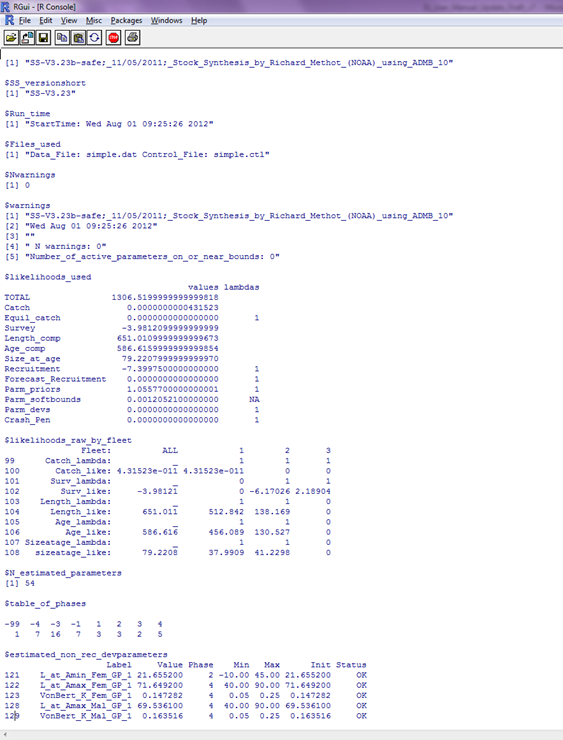
\includegraphics{r4ss_output}
\end{center}
\hfil\\
\hfil\\
\hfil\\
\hfil\\
Example of the plots created using the SS\_plots function:
\begin{center}
	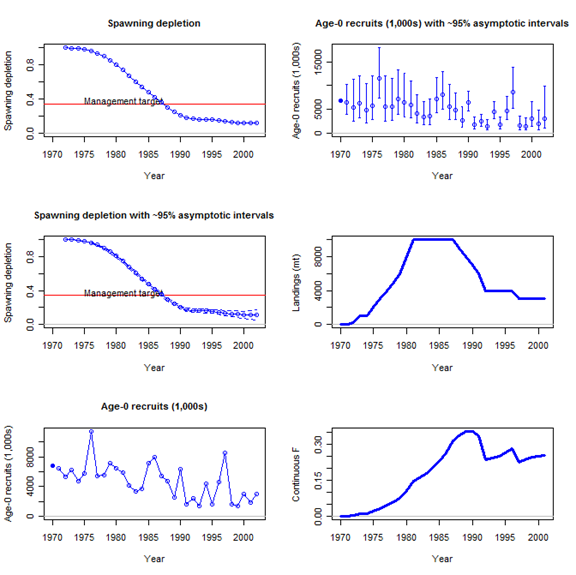
\includegraphics{r4ss_plots}
\end{center}

The functions included in r4ss ranging from general use to functions developed for specific model applications:
\begin{center}
	\begin{longtable}{p{3cm} p{12cm}}
		Core Functions & \\
		\hline
		SS\_output & A function to create a list object for the output from Stock Synthesis\\
		SS\_plots  & Plot many quantities related to output from Stock Synthesis\\
		\hline
		\\
		\multicolumn{2}{l}{Plot functions called by SS\_plots} \\
		\hline
		SSplotBiology & Plot biology related quantities \\
		SSplotCatch   & Plot catch related quantities \\
		SSplotCohorts & Plot cumulative catch by cohort \\
		SSplotComps   & Plot composition data and fits \\
		\hline
	\end{longtable}
\end{center}
